% =================================================================================================
% File:			gestione_contenuti.tex
% Description:	Definisce la sezione relativa ad un capitolo del documento
% Created:		2015-04-25
% Author:		Santacatterina Luca
% Email:		santacatterina.luca@mashup-unipd.it
% =================================================================================================
% Modification History:
% Version		Modifier Date		Change											Author
% 0.0.1 		2015-05-245			inizio stesura sezione capitolo					Santacatterina Luca
% =================================================================================================
%

% CONTENUTO DEL CAPITOLO

\section{Gestione contenuti} % (fold)
\label{sec:gestione_contenuti}


	\subsection{Menu amministratore}
	\label{sec:menu_amministrazione}
		Dopo aver eseguito le istruzioni per l'autenticazione\gloss{} (Capitolo \ref{sec:autenticazione_utente}) viene visualizzata la dashboard\gloss{} dell’applicazione (Figura: \ref{fig:dashboard}).\newline
		Nella schermata principale della dashboard\gloss{} vengono visualizzati in riquadri le \textbf{recipes}\gloss{} disponibili nel sistema (Figura: \ref{fig:dashboard}, rif. 1), mentre nella sinistra dell'applicazione è disponibile il menù principale di gestione (Figura: \ref{fig:menu_principale_utente}).
		\begin{figure}[H]
			\centering
			\centerline{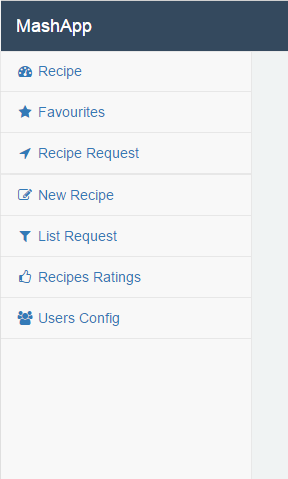
\includegraphics[width=6cm]{images/menu_principale_amministratore.png}}
			\caption{Menù principale amministratore}
			\label{fig:menu_principale_utente}
		\end{figure}
	%section Menu amministratore (end)


% section Gestione contenuti (end)